\documentclass[12pt]{article}
\usepackage{pagecolor,lipsum}
\usepackage{graphicx}
\usepackage{authblk}
\usepackage{setspace}
\usepackage{mathtools}
\usepackage{verbatim}
\usepackage{array}
\usepackage{fancyhdr}
\usepackage{chngcntr}
\usepackage{secdot}
\usepackage{listings}
%\usepackage[dvipsnames]{xcolor}
\sectiondot{subsection}
\setlength{\parindent}{0cm}
\counterwithout{subsection}{section}
\usepackage{courier}
\lstset{basicstyle=\ttfamily}
\newcommand*{\rom}[1]{\expandafter\@slowromancap\romannumeral #1@}
\usepackage[left=2cm, top=2cm, text={17cm, 24cm}]{geometry}
\usepackage[%  
    colorlinks=true,
    pdfborder={0 0 0},
    linkcolor=blue
]{hyperref}
\definecolor{comment}{rgb}{0.16, 0.5, 0.1}
\definecolor{keyw}{rgb}{0.50, 0.20, 0.9}

\onehalfspacing
\pagestyle{fancy}
\fancyhf{}
\lhead{\vspace{6pt}David Mihola}
\rhead{\vspace{6pt}xmihol00}
\chead{\thepage}
\renewcommand{\headrulewidth}{0.5pt}

%%%%%%%%%%%%%%%%%%% TITLE PAGE %%%%%%%%%%%%%
\title{

\includegraphics[scale=0.7]{logo.png}\\
\Huge{Protokol k projektu do předmětu ISS}
}
\author{David Mihola (xmihol00)}
\date{4. 1. 2021}
\newpage
\begin{document}
\pagecolor{white}
	\maketitle
	\thispagestyle{empty}
	\newpage
\section*{Úvod}
\hspace{1.5em}Projekt jsem vypracoval ve skriptovacím jazyce \texttt{Python 3.8.5} s použitím knihoven\\ \texttt{matplotlib, numpy, scipy.io} a \texttt{scipy}. Jelikož je toto první projekt, který jsem psal v jazyce Python, pravděpodobně má implementace nebude využívat veškerých možností tohoto jazyka a nebude zdaleka optimální.

\hspace{1.5em}Programovou část projektu jsem rozdělil do dvou souborů, soubor \texttt{iss\_proj1.py}, ve kterém je převážně implementováno vykreslování grafů, a soubor \texttt{functions.py}, ve kterém je implementována hlavní funkcionalita zahrnující i funkce počítající \texttt{DTF, IDFT} a další.

\hspace{1.5em}Nahrávání jsem prováděl programem \texttt{sox} přes mikrofon od kvalitních sluchátek. Jelikož mám spíše absolutní hudební nesluch, bylo pro mě nahrávání poměrně obtížné. Pro tón "á", který mi přirozeně leží na frekvenci kolem $135\; Hz$, nevycházely moc pěkné spektrogramy ani frekvenční charakteristika roušky, proto jsem zvolil tón "é", který mi přirozeně leží na frekvenci kolem $155\; Hz$.
\section*{Prvotní odhad}
\subsection{Nahrávky tónů}
\begin{center}
\begin{tabular}{| m{0.3\textwidth} | m{0.3\textwidth} | m{0.3\textwidth} |} 
\hline
\textbf{nahrávka} & \textbf{délka v sekundách} & \textbf{délka ve vzorcích}\\
\hline
maskoff\_tone.wav & $4.5$ & $72000$ \\ 
maskon\_tone.wav & $6$ & $96000$\\ 
\hline
\end{tabular}
\end{center}
\subsection{Nahrávky vět}
\begin{center}
\begin{tabular}{| m{0.3\textwidth} | m{0.3\textwidth} | m{0.3\textwidth} |} 
\hline
\textbf{nahrávka} & \textbf{délka v sekundách} & \textbf{délka ve vzorcích}\\
\hline
maskoff\_sentence.wav & $6.25$ & $100000$ \\ 
maskon\_sentence.wav & $6.25$ & $100000$ \\ 
\hline
\end{tabular}
\end{center}
\subsection{Výběr úseků z tónů, vytvoření rámců}
\hspace{1.5em}Vzorec pro výpočet velikosti rámce ve vzorcích:
\begin{center}
$vzorky = F_s \cdot \Delta t$
\end{center}
$\Delta t$ je v tomto případě délka rámce v sekundách a $vzorky$ je výsledný počet vzorků rámce. Pokud dosadíme zadané hodnoty ($F_s = 16000$ a $\Delta t = 0.02$), získáme rámec o délce $320$ vzorků.

\hspace{1.5em}Pro výběr úseků jsem použil metodu cross-korelace. Nejdřív jsem vybral úsek o délce 16160 vzorků (1.01 s) ze začátku nahrávky bez roušky, který jsem porovnal s celou nahrávkou s rouškou. Index, na kterém došlo k největší korelaci, jsem pak zvolil jako střed úseku z nahrávky s rouškou. Rámce pro zobrazení na grafu jsem zvolil taktéž pomocí korelace. Rámce č. 41 s rouškou a bez měly ze 100 vytvořených rámců nevětší korelaci. Rámce jsou vytvořeny funkcí \texttt{create\_frames()}.

\hspace{-4.5em}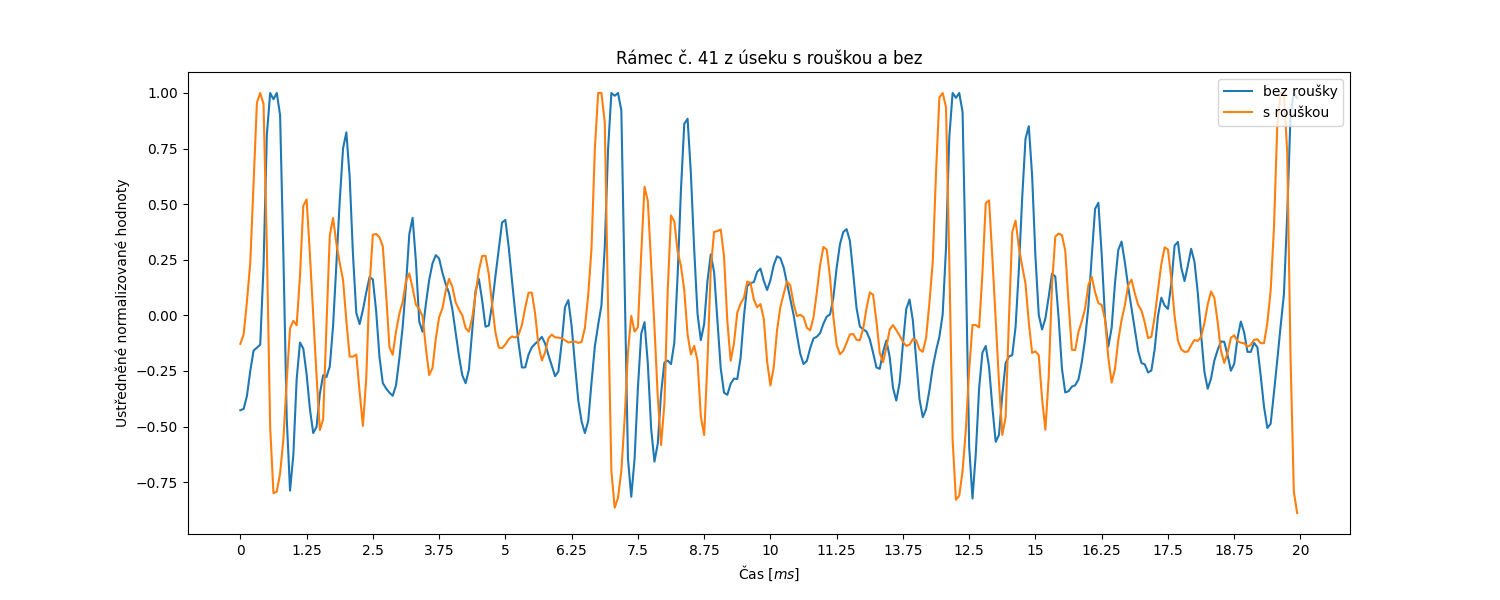
\includegraphics[scale=0.55]{ukol3.png}
\subsection{Kontrola frekvence rámců pomocí klipování a autokorelace}
\hspace{1.5em}Poměrně často se mi stávala chyba dvojitého lagu, tato sada nahrávek je však povedená a na klipovací úrovni $70\%$ se dvojitý lag neprojevuje. Klipovaní a autokorelaci iplmentuje funkce \texttt{clip\_frames()} respektive funkce \texttt{autocorelate()}.

\hspace{1.5em}Pro autokorelaci jsem použil vzorec
\begin{center}
\vspace{-2em}
\[ R[k] = \sum_{n=0}^{N-1-k} s[n]s[n + k] \]
\end{center}
z prezentace\footnote[1]{http://www.fit.vutbr.cz/~grezl/ZRE/lectures/04\_lpc\_en.pdf} od Jana Černockého a Valentina Hubeiky.

\vspace{1em}
\textbf{(a) Grafy:}

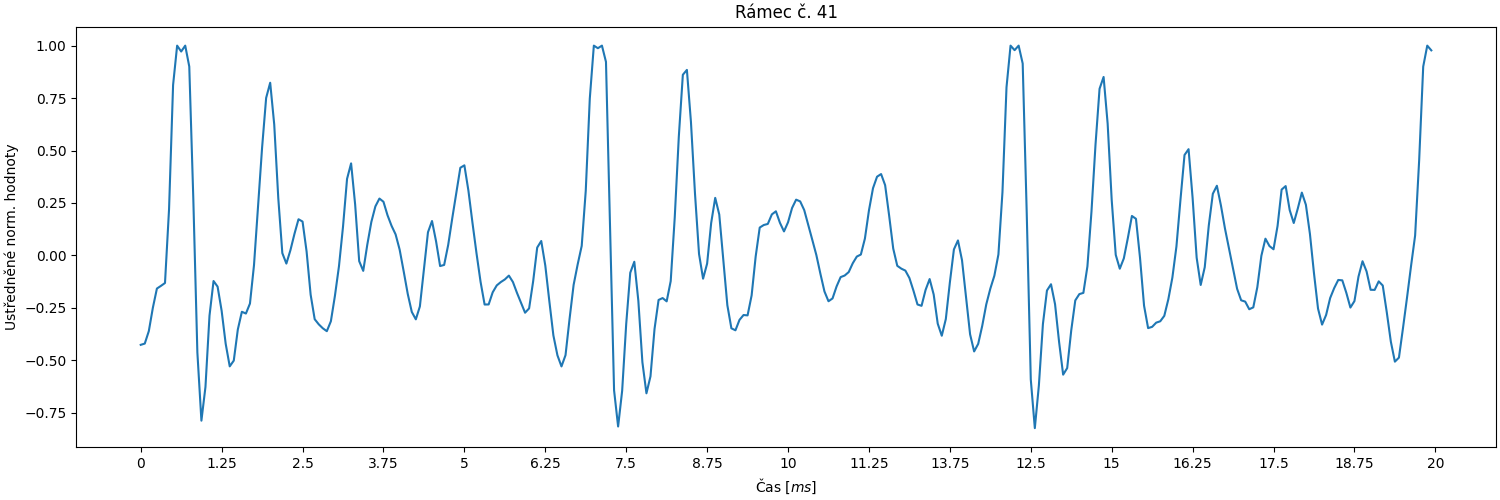
\includegraphics[scale=0.44]{ukol4a.png}

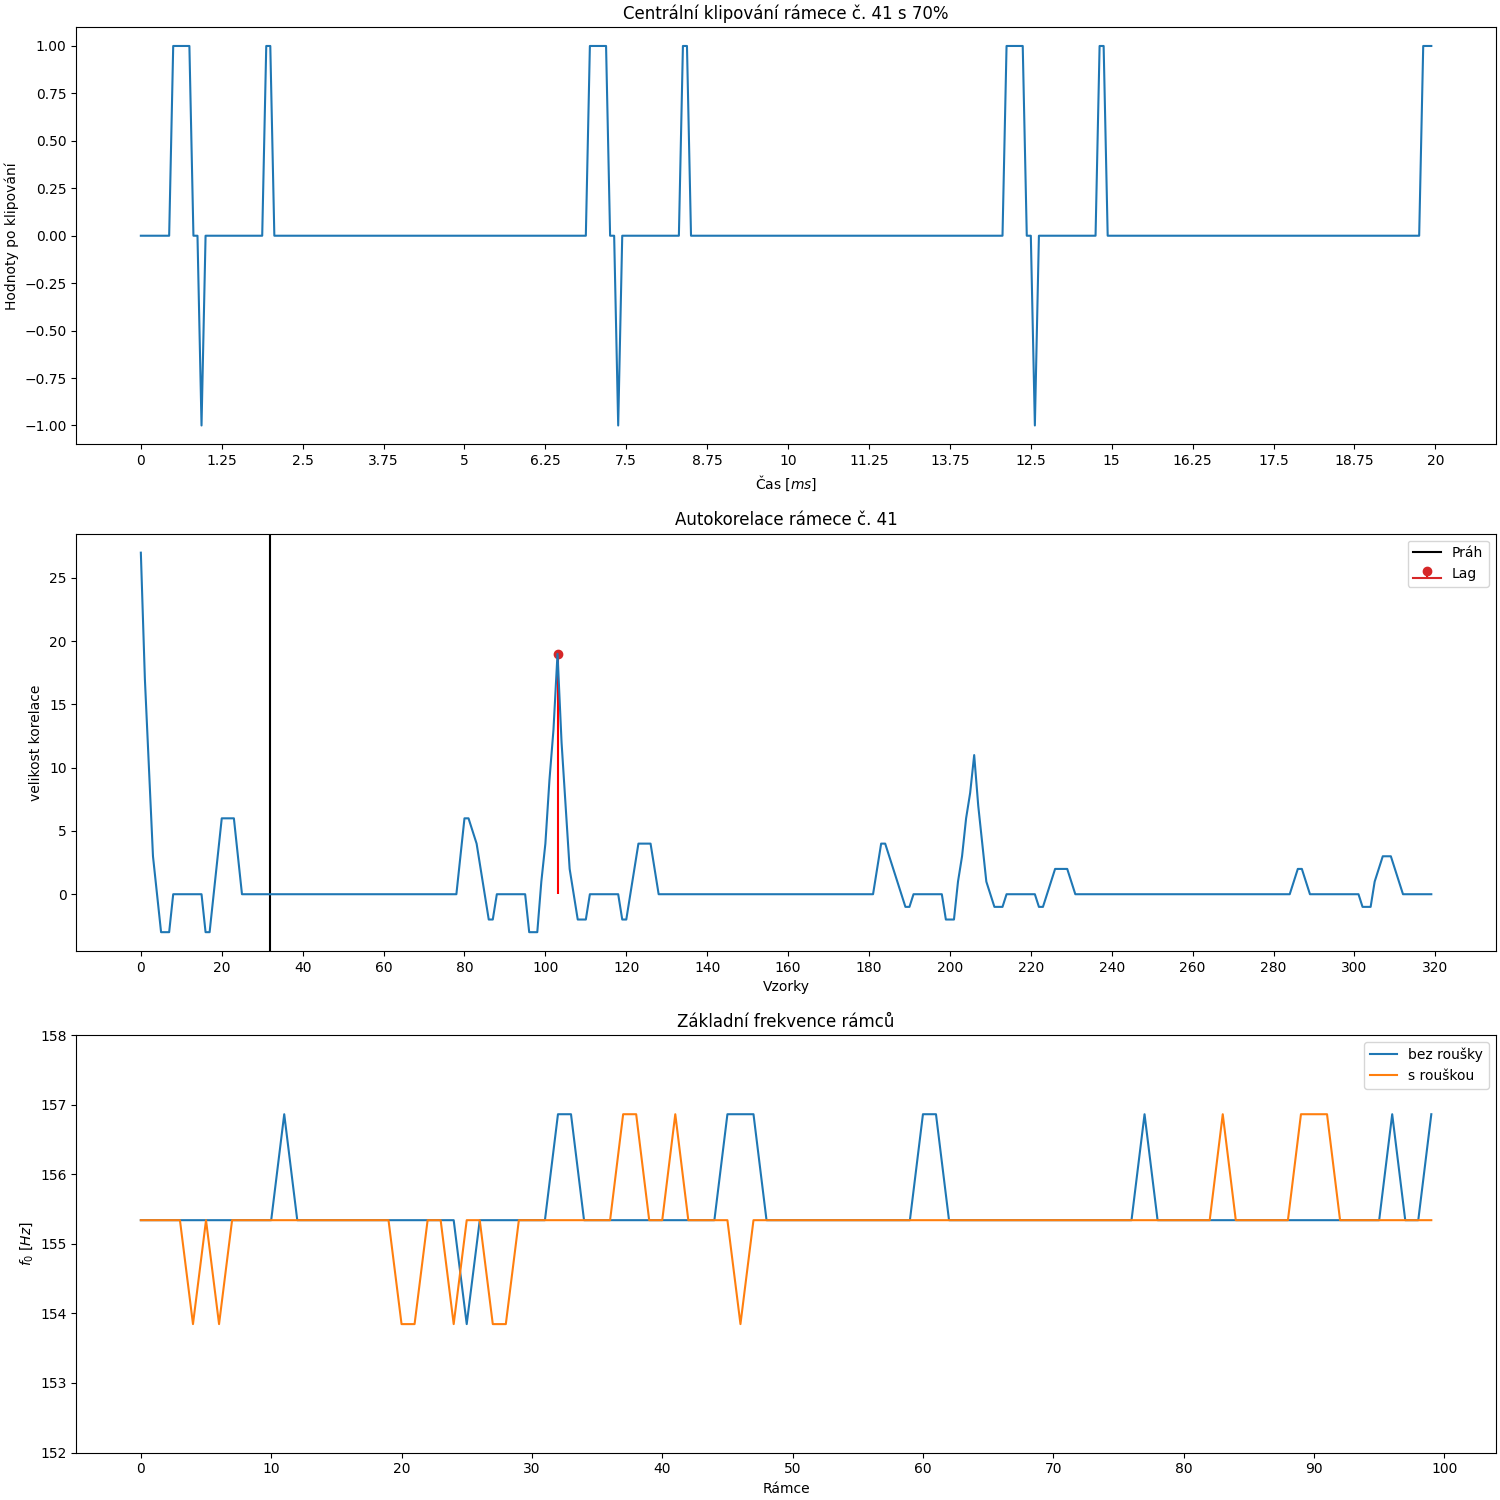
\includegraphics[scale=0.44]{ukol4b.png}

\textbf{(b) Střední hodnota a rozptyl základních frekvencí nahrávek:}
\begin{center}
\begin{tabular}{| m{0.3\textwidth} | m{0.3\textwidth} | m{0.3\textwidth} |} 
\hline
\textbf{nahrávka} & \textbf{střední hodnota základní frekvence v $Hz$} & \textbf{rozptyl základní\newline frekvence v $Hz^2$}\\
\hline
bez roušky & $155.49239$ & $0.25416$ \\ 
s rouškou & $155.32692$ & $0.34067$\\ 
\hline
\end{tabular}
\end{center}
\vspace{1em}
\textbf{(c) Výpočet a možné zmenšení velikosti změny $f_0$:}

\hspace{1.5em}Pro výpočet základní frekvence $f_0$ jsem použil tento vzorec.
\begin{center}
$f_0 = \frac{F_s}{lag}$
\end{center}
Ze vzorce je patrné, že velikost změny frekvence $f_0$ závisí na velikosti $F_s$ (vzorkovací frekvenci). Velikost změny $f_0$ při změně lagu o $\pm 1$ lze tak zmenšit nahráváním na vyšší vzorkovací frekvcenci. Pro třikrát vyšší vzorkovací frekvenci ($48 000\; kH$) pak získame třikrát více vzorků na rámec, tím pádem i třikrát menší změnu $f_0$ s posunem lagu o $\pm 1$ (vzorkovací frekvenci $16000\; Hz$ odpovídá posun lagu o $\pm 3$). Nahrávání na vyšší vzorkovací frekvenci nemusí být vždy hardwarově možné, pak už můžeme změnu $f_0$ ovlivnit pouze softwarově, např. nadvzorkováním pomocí interpolace\footnote[2]{http://poseidon2.feld.cvut.cz/courses/CS/web/CS/Prednasky/Pred5.pdf}.

\subsection{Převod z časové domény do frekvenční pomocí DFT}
\textbf{(a) Funkce implementující DFT:}

\hspace{1.5em}Oproti knihovní funkci implementující DTF (\texttt{np.fft.fft()}) je mnou implementovaná DFT značně pomalejší, přesněji FFT pracuje v linearitmické časové složitosti, kdežto DFT pracuje ve složitosti kvadratické. Funkce současně počítá DFT pro všechny rámce bez roušky i s rouškou. Tělo DFT je implementováno podle známého vzorce.
\begin{center}
\vspace{-2em}
\[ X[k] = \sum_{n=0}^{N-1} x[n]e^{-j\frac{2\pi}{N}kn} \]
\vspace{-2em}
\end{center}
\begin{lstlisting}[language=Python]
def calculate_DFT(frames_off, frames_on, frames_count):
  DFT_off = []
  DFT_on = []
  for i in range(0, frames_count):
    frame_dft_off = []
    frame_dft_on = []
    for k in range(0, 1024):
      sum_off = 0 + 0j
      sum_on = 0 + 0j
      for n in range(0, 320): # pro n od 320 do 1024 je hodnota vzdy 0
        e_pow = np.e**(-1j*2*np.pi/1024*n*k) # vypocet imaginarni casti
        sum_off += frames_off[i][n]*e_pow
        sum_on += frames_on[i][n]*e_pow
      frame_dft_off.append(sum_off)
      frame_dft_on.append(sum_on)
    DFT_off.append(frame_dft_off)
    DFT_on.append(frame_dft_on)
  return DFT_off, DFT_on
\end{lstlisting}
\newpage
\textbf{(b) Spektrogramy:}

Pro zobrazení spektrogramů jsem použil funkci: \texttt{plt.pcolormesh()}. Aby byly spektrogramy zobrazeny správně, transponoval jsem matici výsledků DFT takto: \begin{lstlisting}[language=Python] 
[list(i) for i in zip(*[Spect_off[j] for j in range(0, frames_count)])]
\end{lstlisting}
Na spektrogramech lze dobře vidět, že největší výkon má signál na násobcích základní frekvence ($f_0 = 155\;Hz$). Dále si můžeme všimnout, že oblast s největším výkon ($620\;Hz$ a $775\; Hz$) signálu bez roušky se na signálu s rouškou objevuje na dvojnásobných frekvencích ($1240\;Hz$ a $1395\; Hz$). Zároveň došlo na spektrogramu s rouškou k nepatrnému zostření pruhů s největším výkonem (zejména na vyšších frekvencích), v tomto směru bych čekal spíše opačný efekt.

\hspace{-0.7cm}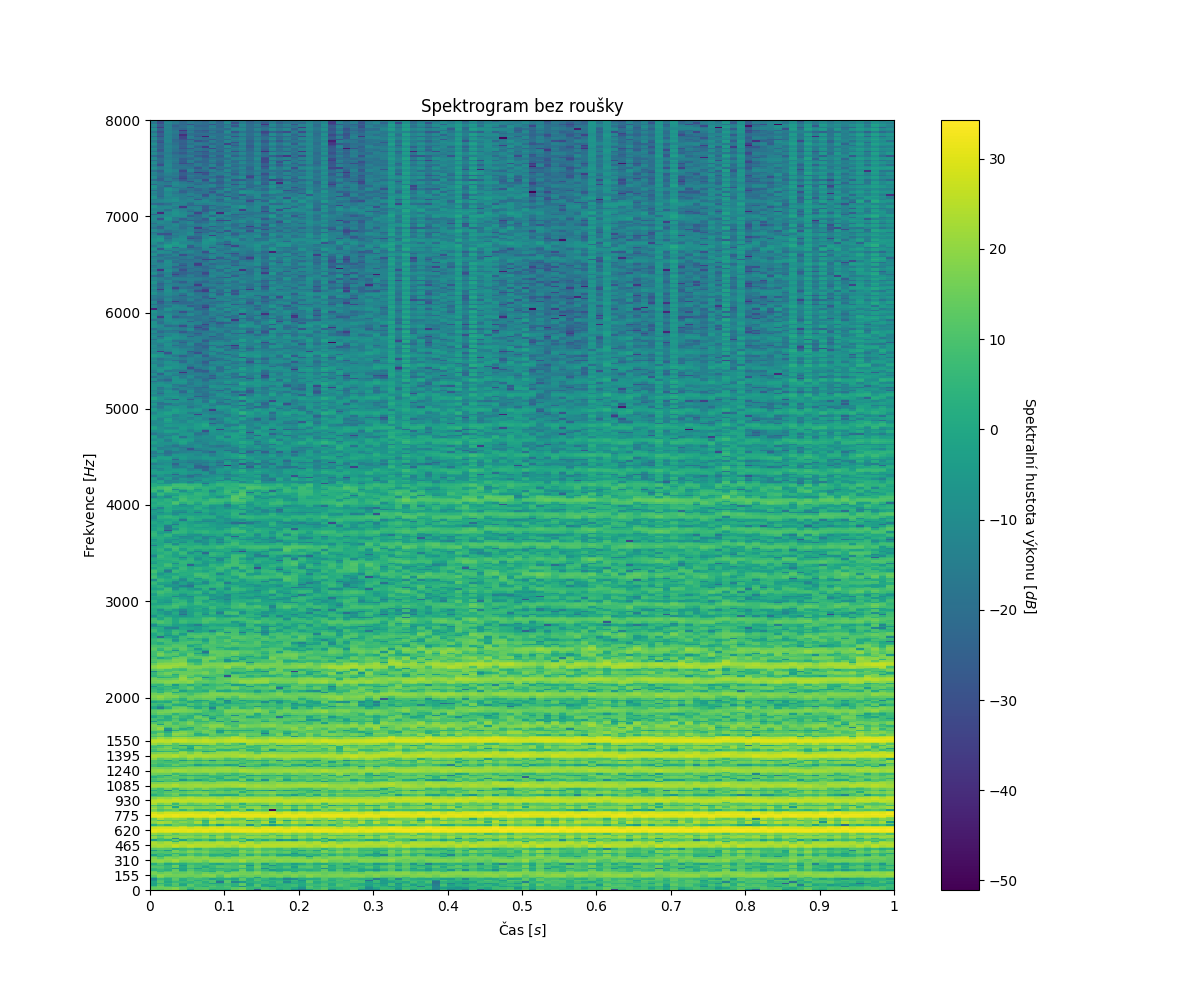
\includegraphics[scale=0.65]{nomask_spec.png}

\hspace{-0.7cm}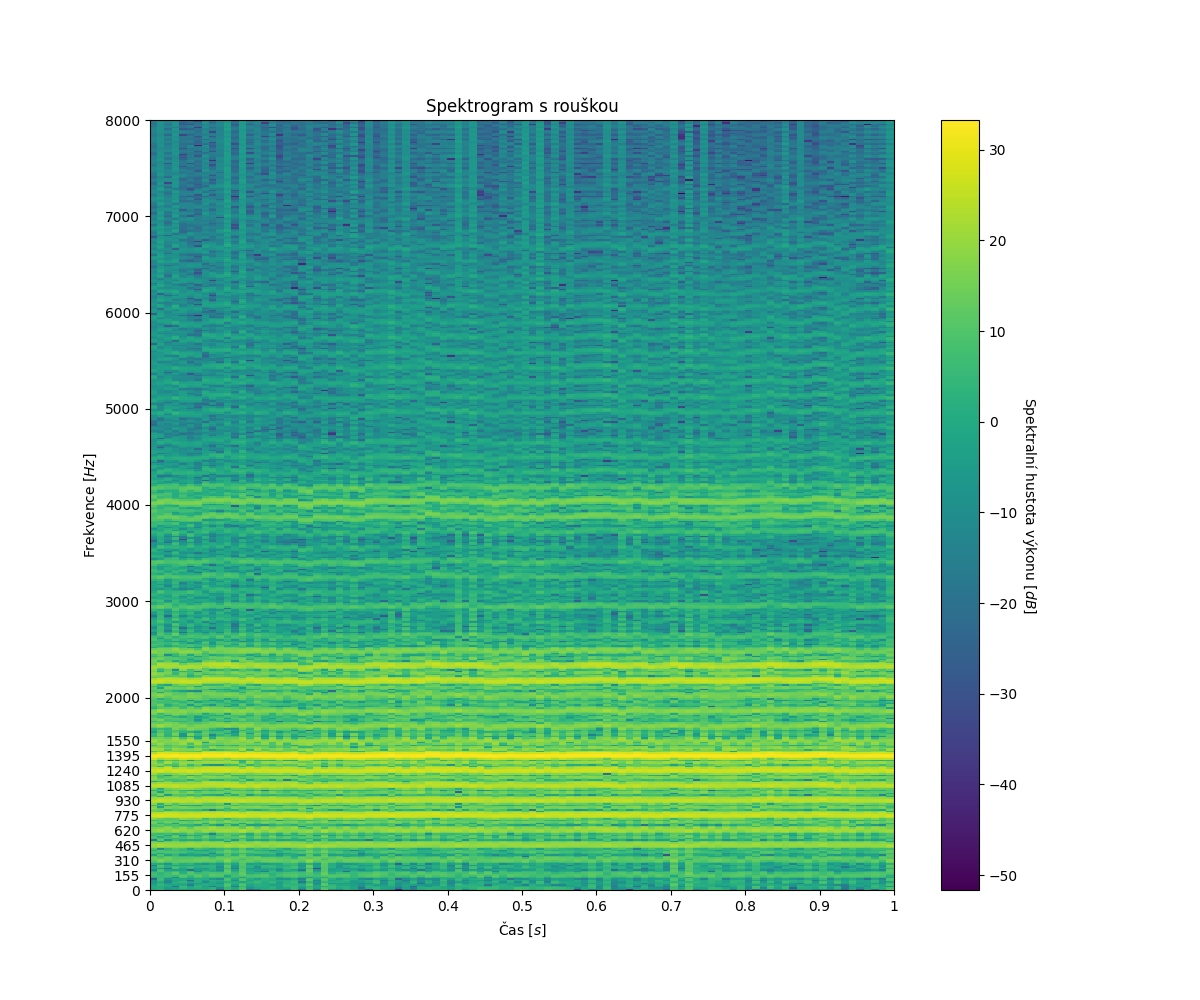
\includegraphics[scale=0.65]{mask_spec.png}
\subsection{Frekvenční charakteristika roušky}
\textbf{(a) Vztah pro výpočet $H(e^{j \omega})$:}

\hspace{1.5em} Jelikož při výpočtu DFT jsem již provedl \texttt{z-transformaci} jak na vstupní signál (bez roušky), tak na výstupní signál (s rouškou), mužeme nyní pro výpočet frekvenční charakteristiky použít přenosovou funkci,
\begin{center}
$H(z)= \frac{Y(z)}{X(z)}$
\end{center}
kde pouze nahradíme $z$ za $e^{j \omega}$ a získáme vztah implementovaný funkcí \texttt{freqv\_char()}
\begin{center}
$H(e^{j \omega})= \frac{Y(e^{j \omega})}{X(e^{j \omega})}=\frac{DFT\_mask\_on}{DFT\_mask\_off}$
\end{center}

\newpage
\textbf{(b) Graf frekvenční charakteristiky:}

\hspace{-4.5em}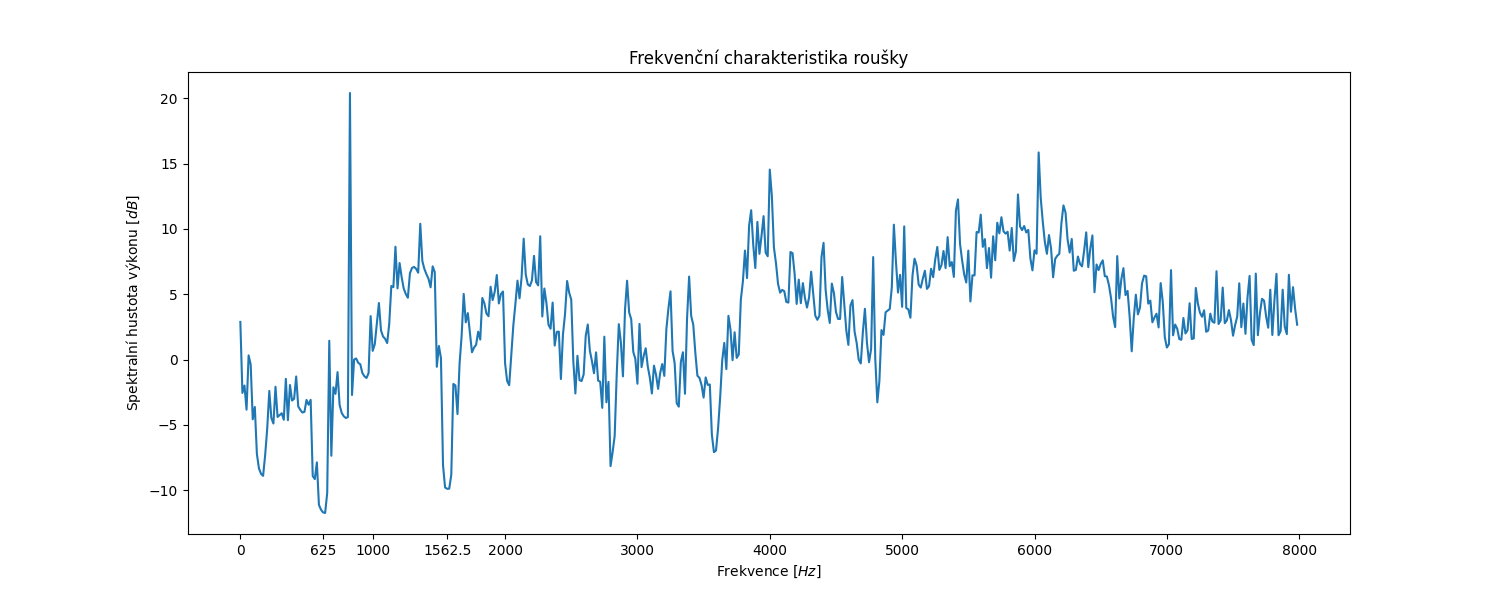
\includegraphics[scale=0.55]{ukol6.png}

\textbf{(c) Komentář k filtru:}

\hspace{1.5em}Jedná se o FIR filter, čímž je zaručena jeho stabilita. Z frekvenční charakteristiky lze usoudit, že filter bude mít vlastnosti několikanásobné pásmové zádrže, zejména na frekvencích kolem $625\; Hz$ a $1562.5\; Hz$, ale i na frekvencích kolem $150\; Hz$, $2800\; Hz$ a $4650\; Hz$. Zajímavé je, že všechny tyto zádrže jsou právě na násobcích základní frekvence ($f_0 = 155\; Hz$). Z toho usuzuji, že filter nebude mít očekávané vlastnosti. Další důvod, proč filter asi nebude fungovat úplně správně, je ten, že poměrně značná část spektra je kladná, tudíž filter bude mít tendenci zhlasovat.

\subsection{Návrat do časové domény}
\textbf{(a) Implementace IDFT:}

\hspace{1.5em}Opět je má implementace IDFT s $1024 \cdot 1024 = 1048579$ výpočty vzorce značně pomalejší než algoritmus IFFT, který provede pouze $1024 \cdot log_2(1024) = 10240$ výpočtů vzorce.

\begin{lstlisting}[language=Python]
def calculate_IDFT(freqv_avg):
  Filter = []
  for n in range(0, 1024):
    s = 0 + 0j
    for k in range(0, 1024):
      s += freqv_avg[k]*np.e**(1j*2*np.pi/1024*n*k)
    s /= 1024
    Filter.append(s)
    
  return Filter
\end{lstlisting}

\textbf{(b) Graf impulsní odezvy roušky:}

\hspace{-4.5em}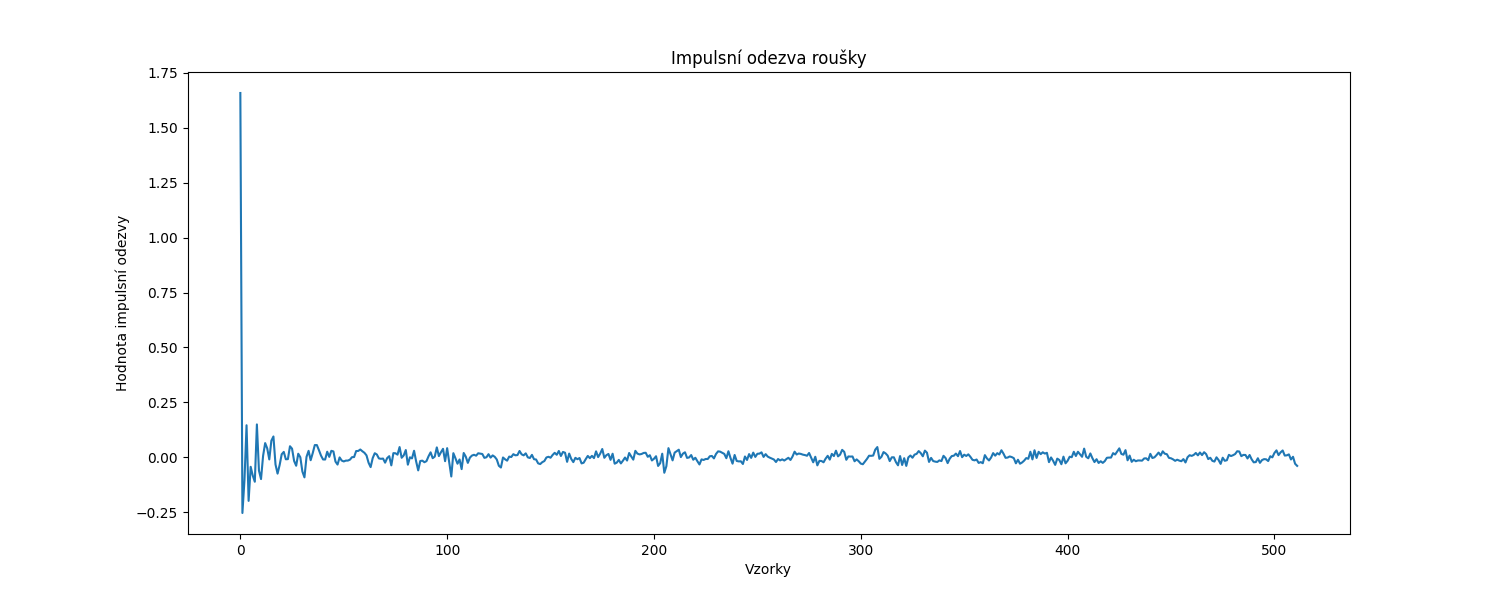
\includegraphics[scale=0.55]{impuls_resp.png}
\subsection{Aplikace filtru}
\hspace{1.5em}Jak už jsem avizoval v úkolu č. 6, nejvíce se filter projeví zvýšením hlasitosti nahrávky. Možná to nakonec nebude špatně, věta s rouškou je převážně hlasitější než věta bez roušky, aniž bych se o to nějak úmyslně pokoušel. Vysvětluji si to tím, že při mluvení s rouškou se hůře slyším, tudíž mluvím hlasitěji. Stejná situace nastala nejspíše i u nahrávek tónů, i když tam by se rozdíly v hlasitosti měly potlačit normalizací.

\hspace{1.5em}Nejméně se nahrávky s rouškou a se simulovanou rouškou podobají od začátku po $20000$ vzorků a na konci od $83000$ do $95000$ vzorků, paradoxně v těchto úsecích si jsou naopak nahrávky s rouškou a bez ní podobné nejvíce.

\hspace{1.5em}Naopak ve středu nahrávky od $20000$ do $83000$ vzorků filter poměrně dobře zafungoval a nahrávky s rouškou a se simulovanou rouškou jsou si velmi podobné. Přiblíženě se o tom můžeme přesvědčit na posledním grafu, na kterém jsou všechny nahrávky zachyceny v rozmezí od $63500$ do $64500$ vzorků.

\hspace{1.5em}Aplikaci filtru jsem provedl knihovní funkcí \texttt{scipy.signal.lfilter()}.

\newpage
\textbf{(a) Grafy nahrávek:}

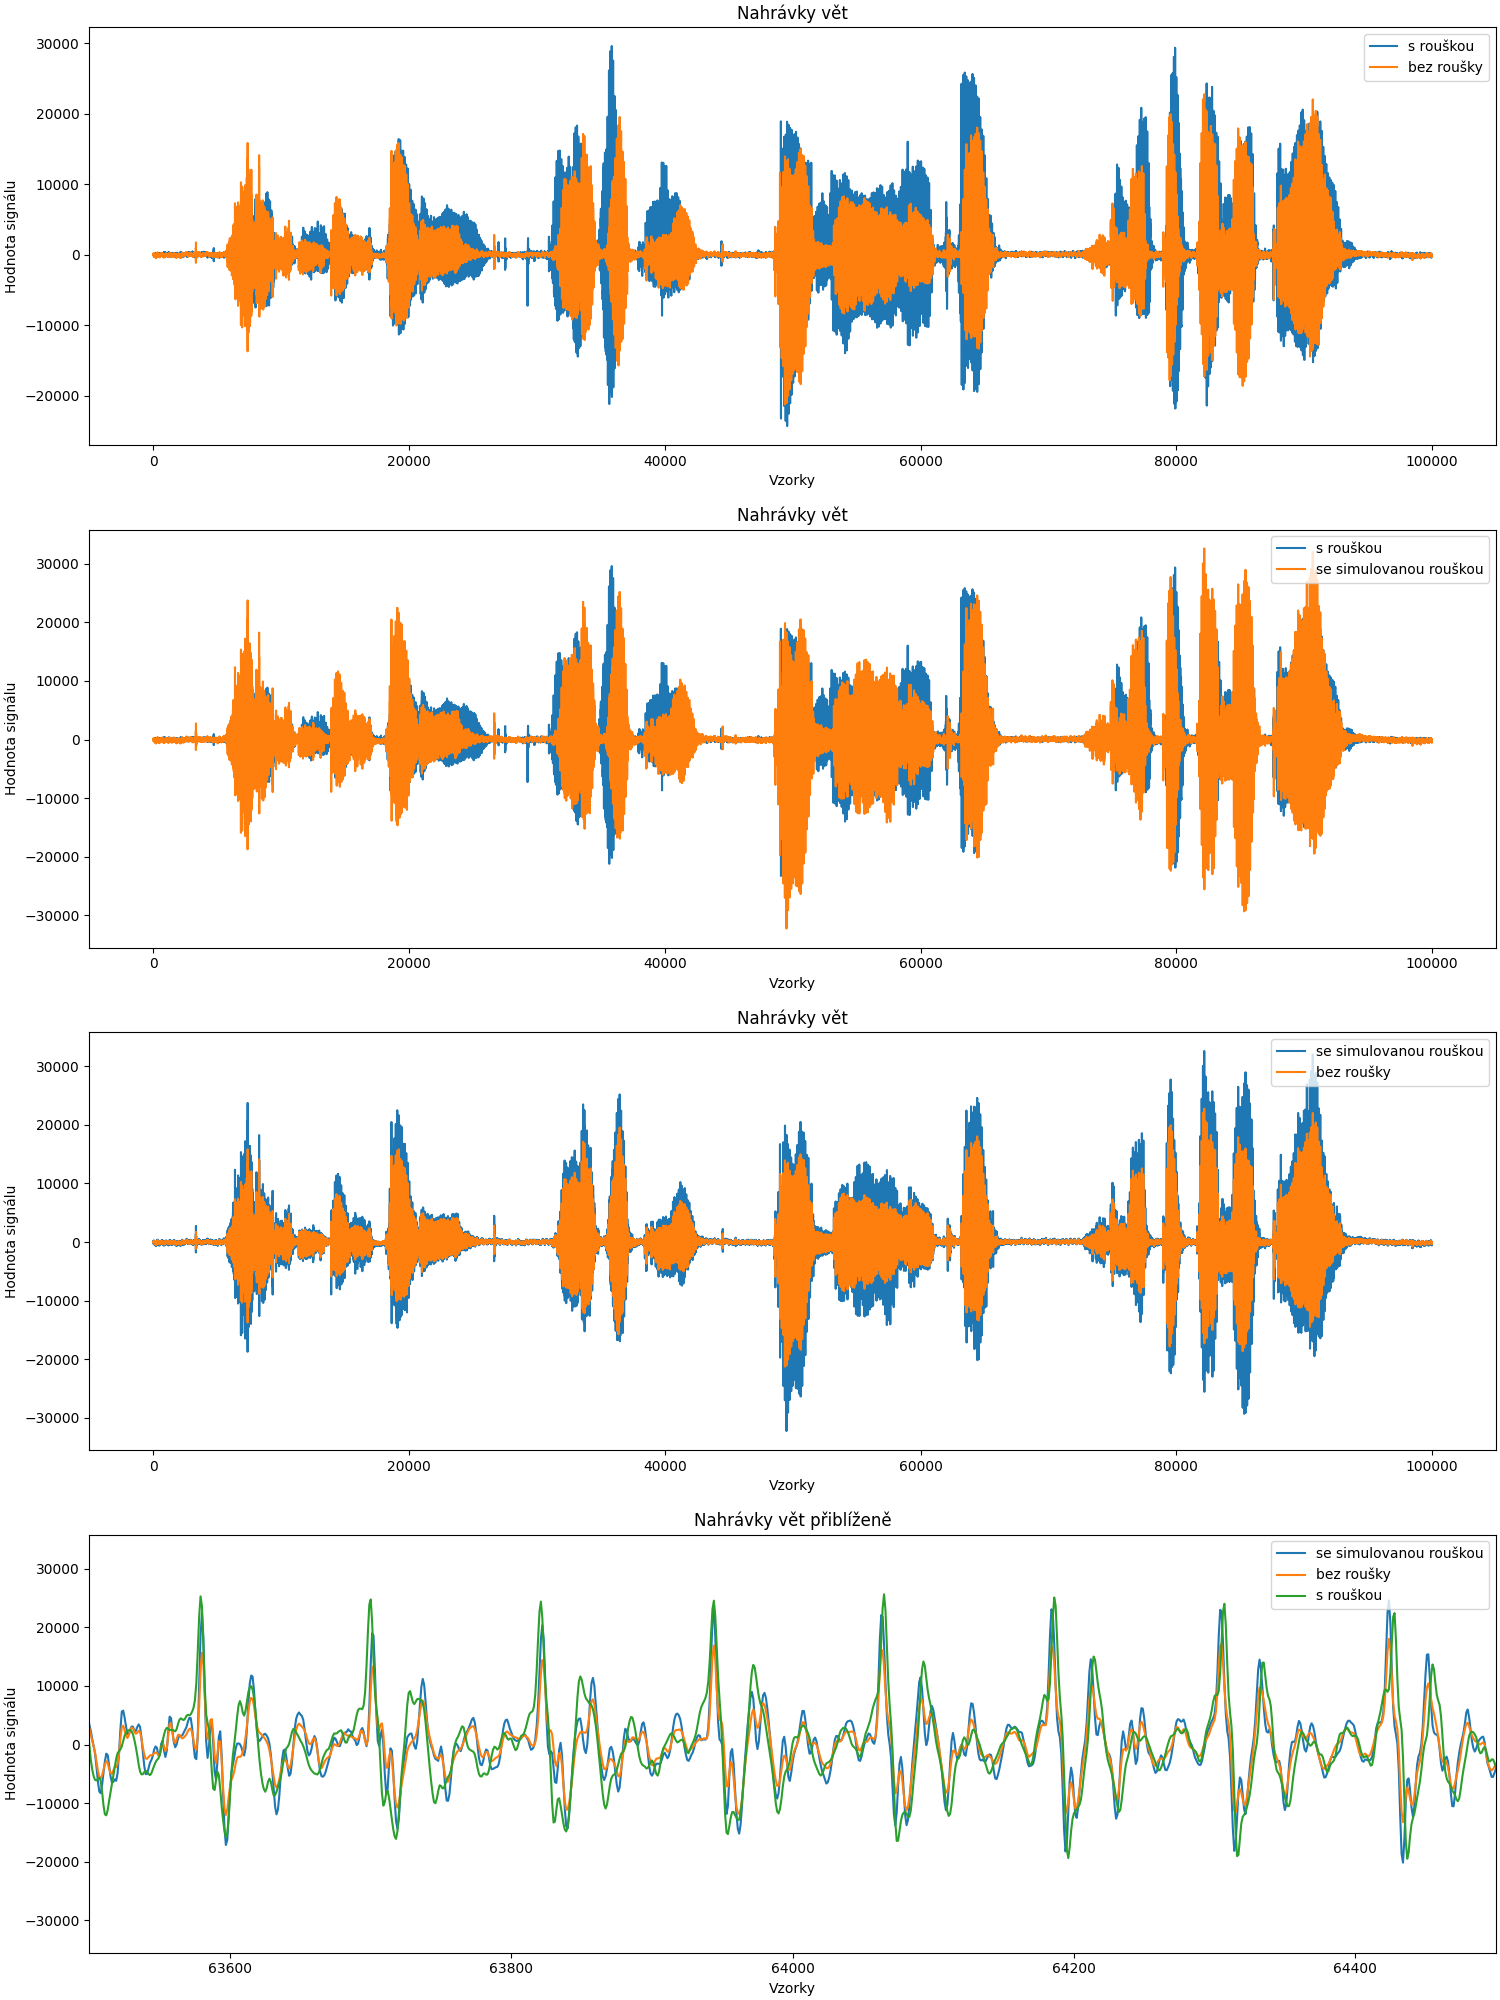
\includegraphics[scale=0.44]{ukol8.png}

\subsection{Závěr}
\hspace{1.5em}Po nemalém usílí se mi povedlo nahrát dvě nahrávky tónů na téměř stejné základní frekvenci $155\;Hz$, která je patrná ze spektrogramů. Stejně tak se mi podařilo nahrát i v celku podobné věty. Jediný problém nahrávek je nejspíše jejich hlasitost, která ovlivňuje výsledek.

\hspace{1.5em}Části implementace od kontroly frekvence rámců, jejich klipování a autokorelaci po vytvoření spektrogramů odpovídají ukázkám ze zadání, považuji je tedy za úspěšné.

\hspace{1.5em}Za úspěšné považuji i části, ve kterých vytvářím frekvenční charakteristiku roušky (před zprůměrováním rámců jsem provedl kontrolu funkcí \texttt{signal.freqz()}), převod zpět do časové domény (opět proběhla kontrola s knihovovní funkcí \texttt{np.fft.ifft()}) i aplikaci filtru.

\hspace{1.5em}Ačkoliv jsem v programové části doufejme neprovedl žádné chyby, výsledné simulace nahrávek tomu moc neodpovídají. U věty jde rouška slyšet jen minimálně. U tónu je to ještě horší, zde dochází k přílišnému zhlasení a tón je tak poškozený.

\hspace{1.5em}Celkově projekt musím ohodnotit zatím jako jeden z nejtěžších, se kterými jsem se po dobu svého studia na VUT setkal. Řadím ho ale také k jednomu z nejužitečnějších a nejzajímavějších.

\newpage
\section*{Doplňující úkoly}
\subsection{Filtrace metodou overlap-add}
\hspace{1.5em}U implementace metody overlap-add jsem zvolil nejdříve převod do frekvenční domény pomocí FFT, pak provedl násobení, které by jinak v časové doméně znamenalo konvoluci, a následně jsem provedl opět převod do časové domény pomocí IFFT a správně přičetl výsledky do vytvářeného filtrovaného signálu. Převod do frekvenční domény a následně zase zpět se může zdát zbytečný a časově neoptimální, není tomu ale tak. FFT a IFFT pracují natolik rychle, že je výhodnější provést převod a poté jen násobení ve frekvenční doméně namísto operace konvoluce (násobení a sumování) v doméně časové. 

\hspace{1.5em}Stejným způsobem provádí konvoluci i knihovní funkce. Není tedy divu, že po filtraci metodou overlap-add, je simulovaná nahrávka totožná se simulovanou nahrávkou vytvořenou knihovní funkcí \texttt{scipy.signal.lfilter()}.

\vspace{1em}
\textbf{(a) Funkce aplikující filter na signál metodou overlap-add:}

\begin{lstlisting}[language=Python]
def overlap_add(flter, signal, fft_n):
  f_len = len(flter)  # delka filtru
  s_len = len(signal) # delka filtrovaneho signalu
  step = fft_n - f_len + 1 # delka jehnoho kroku
  filer_FFT = np.fft.fft(flter, n=fft_n)
  res = [0]*(s_len+fft_n)
  for i in range(0, s_len, step):
    segment = np.fft.ifft(np.fft.fft(signal[i:i+step], n=fft_n)*filer_FFT)
    for j in range(0, fft_n):
      res[i+j] += segment[j].real
    
  return res[0:s_len]
\end{lstlisting}
\subsection{Okénková funkce}
\textbf{(a) Hanningova okénková funkce:}

\hspace{1.5em}Hanningovu okénkovou funkci jsem zvolil na základě více zdrojů, které ji upřednostňovaly pro zpracování řeči\footnote[3]{https://download.ni.com/evaluation/pxi/Understanding\%20FFTs\%20and\%20Windowing.pdf\\ https://dsp.stackexchange.com/questions/36513/applying-a-window-function-to-a-speech-signal\\ http://www.cs.tut.fi/kurssit/SGN-4010/ikkunointi\_en.pdf}. Vytvoření okénkové funkce bylo jednoduché, použil jsem knihovní funkci \texttt{np.hanning()}. Okénkovou funkci jsem poté aplikoval jednoduše v časové doméně pouhým pronásobením s jednotlivými rámci ve funkci \texttt{apply\_window()}.
\newpage
\textbf{(b) Grafy:}

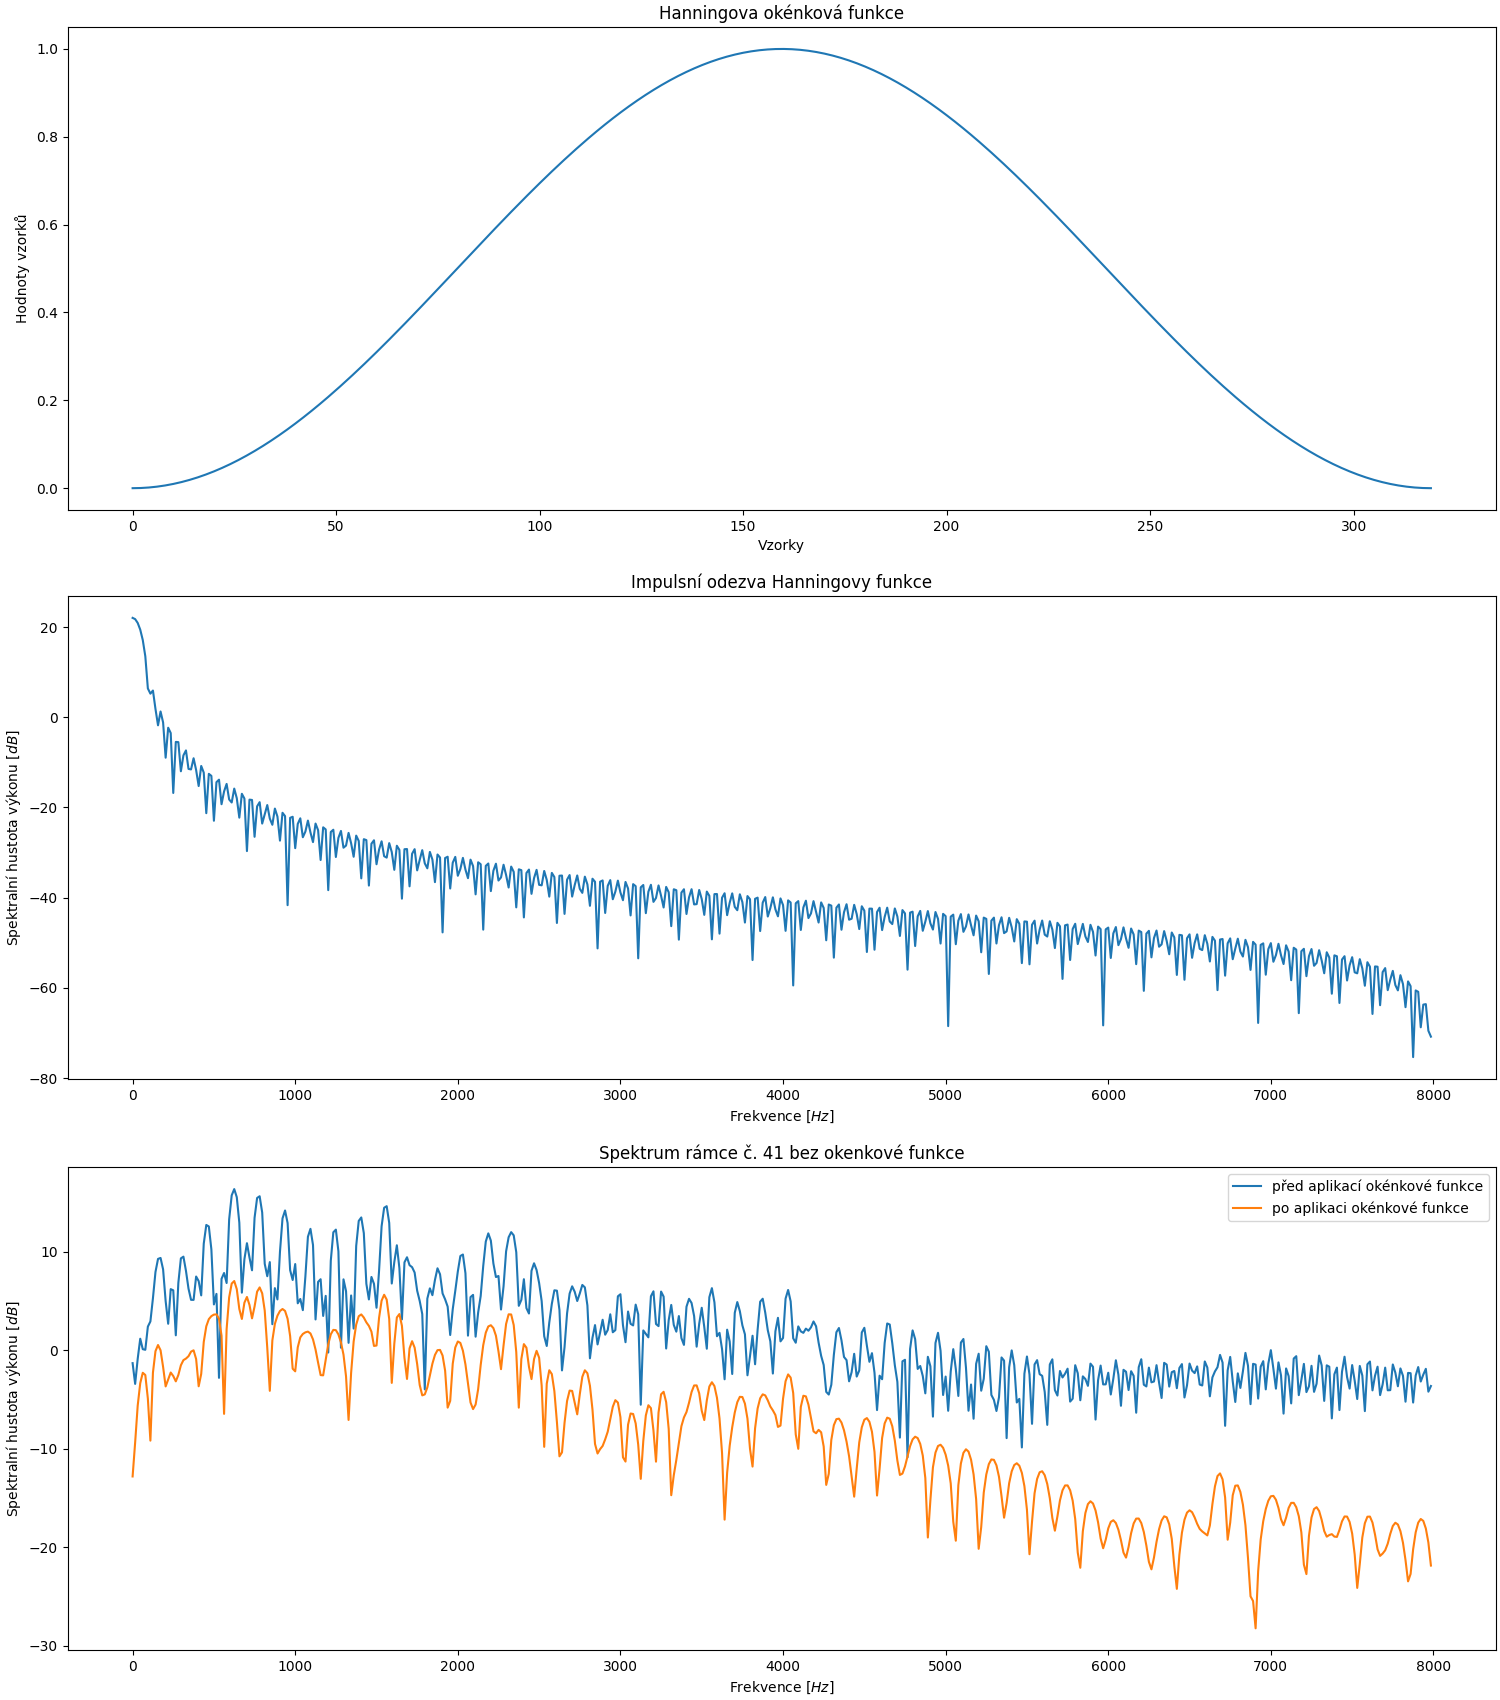
\includegraphics[scale=0.44]{ukol11.png}

\textbf{(c) Porovnání spekter}

\hspace{1.5em}Po aplikaci okénkové funkce dochází k vyhlazení a mírnému posunu spektra. Okénková funkce je užitečná, protože zajišťuje, že je rámec tvořen jednou periodou nějaké funkce, která vznikne násobením původní funkce s okénkovou. Zajištění, aby měl rámec přesně jednu periodu, je nutné pro správné fungování funkce DFT (FFT), která na vstupu očekává jednu periodu periodického signálu.

\subsection{Oprava dvojnásobného lagu}
\hspace{1.5em}Na této sadě nahrávek tónů se dvojnásobný lag při klipovací úrovni $70\%$ neprojevil. Při navýšení této úrovně na $80\%$ se již dvojnásobný lag projevil na rámci s rouškou č. 93.

\vspace{1em}
\textbf{(a) Grafy:}

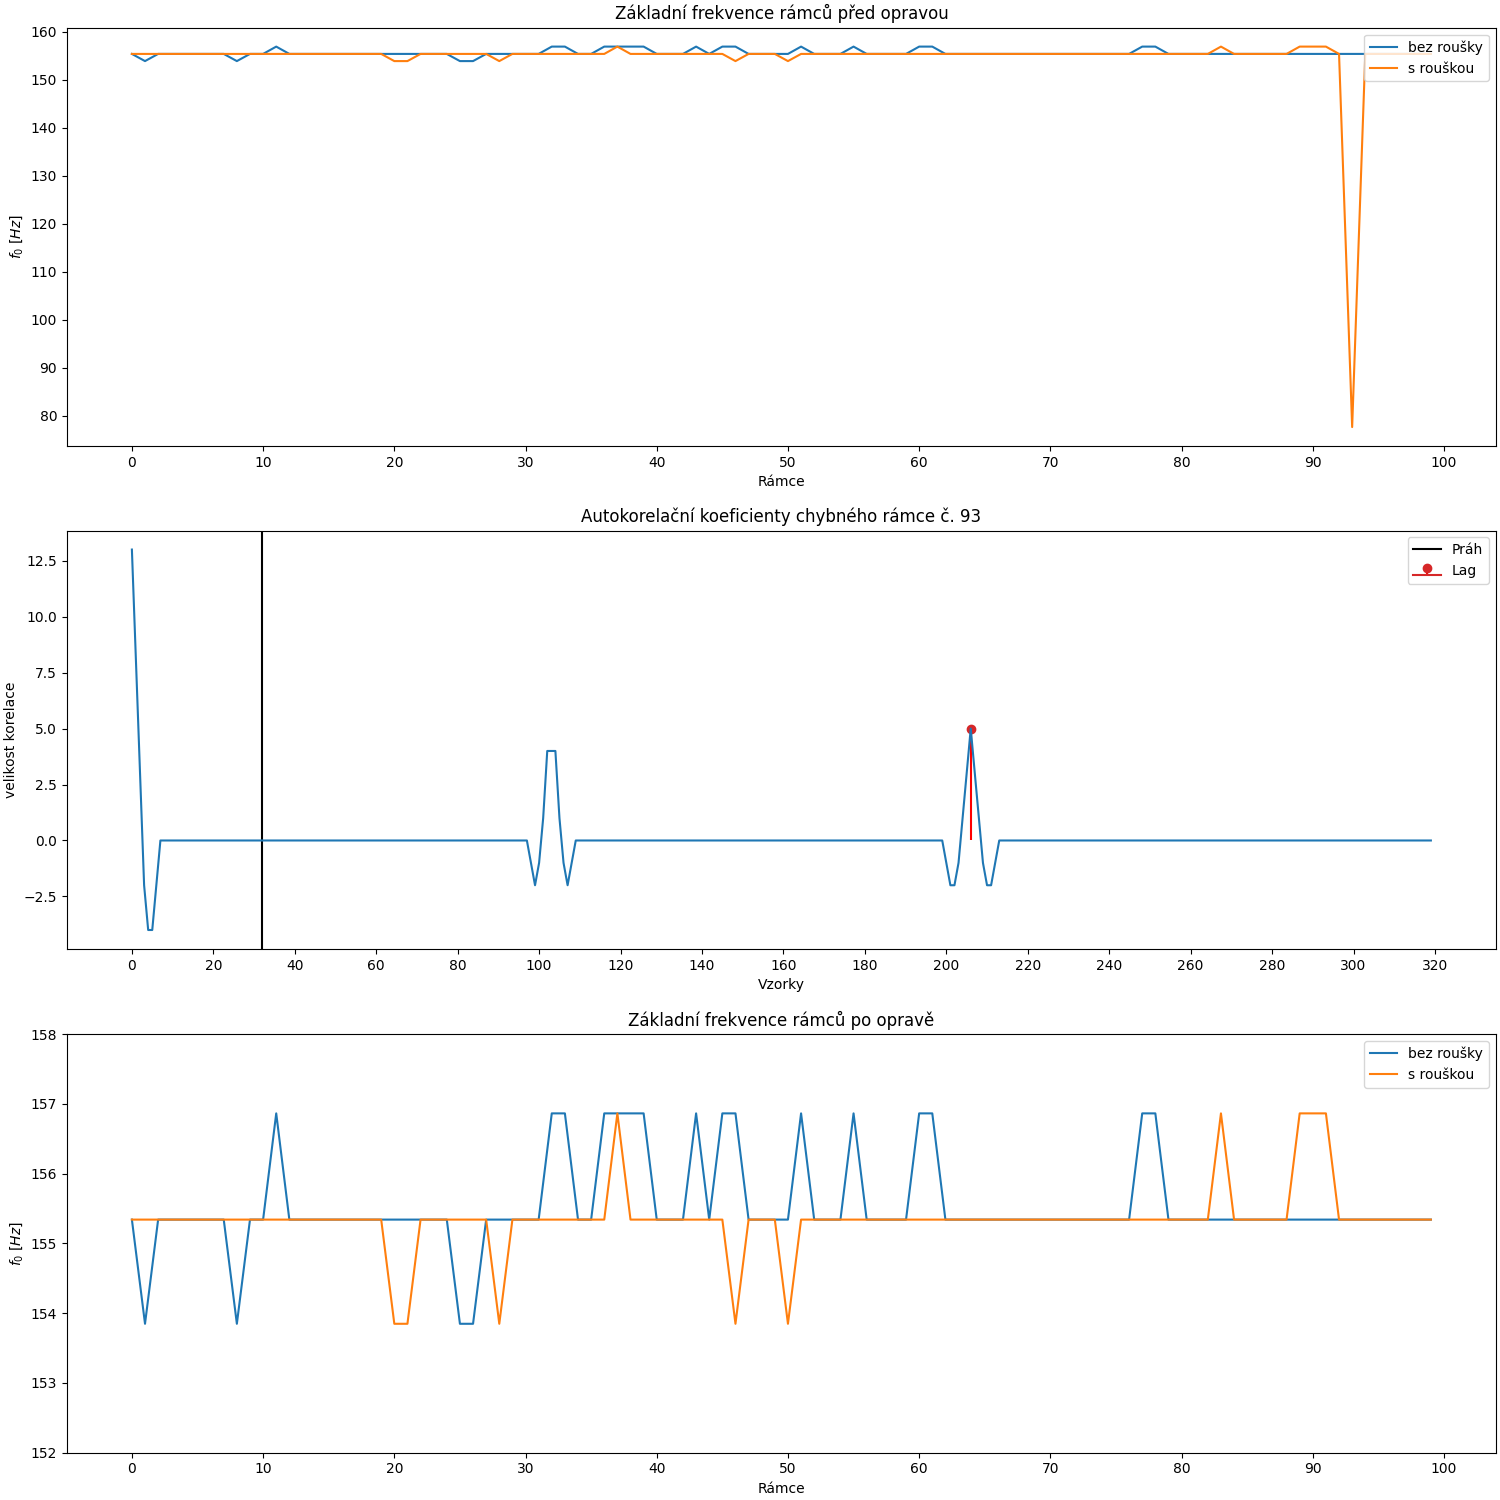
\includegraphics[scale=0.44]{ukol12.png}

\textbf{(b) Popis implementace:}

\hspace{1.5em}Detekci a nápravu rámců s dvojnásobným lagem jsem prováděl až na vypočtených frekvencích jednotlivých rámců. Na chybné rámce jsem použil tzv. mediánový filter. Zároveň jsem si ukládal hodnotu indexu posledního opraveného rámce, jehož korelační koeficienty jsou zobrazeny na grafu. Oprava frekvencí rámců je implementována ve funkci \texttt{correct\_frames()}.

\subsection{Základní tón ze stených rámců}
\hspace{1.5em}Na první pohled je graf frekvenční charakteristiky všech rámců takřka totožný s grafem z rámců, které mají stejnou frekvenci. Rámců se stejnou frekvencí bylo $74$, což je poměrně velký počet a ostatní rámce se liší maximálně o $3\; Hz$. To vysvětluje jen minimální změny. Velmi malých změn si můžeme všimnout na frekvencích kolem $50\;Hz$, $650\;Hz$ a $1000\;Hz$. Výběr rámců se stejnou frekvencí provádí funkce \texttt{same\_freqv\_frames()}.

\vspace{1em}
\hspace{-4.5em}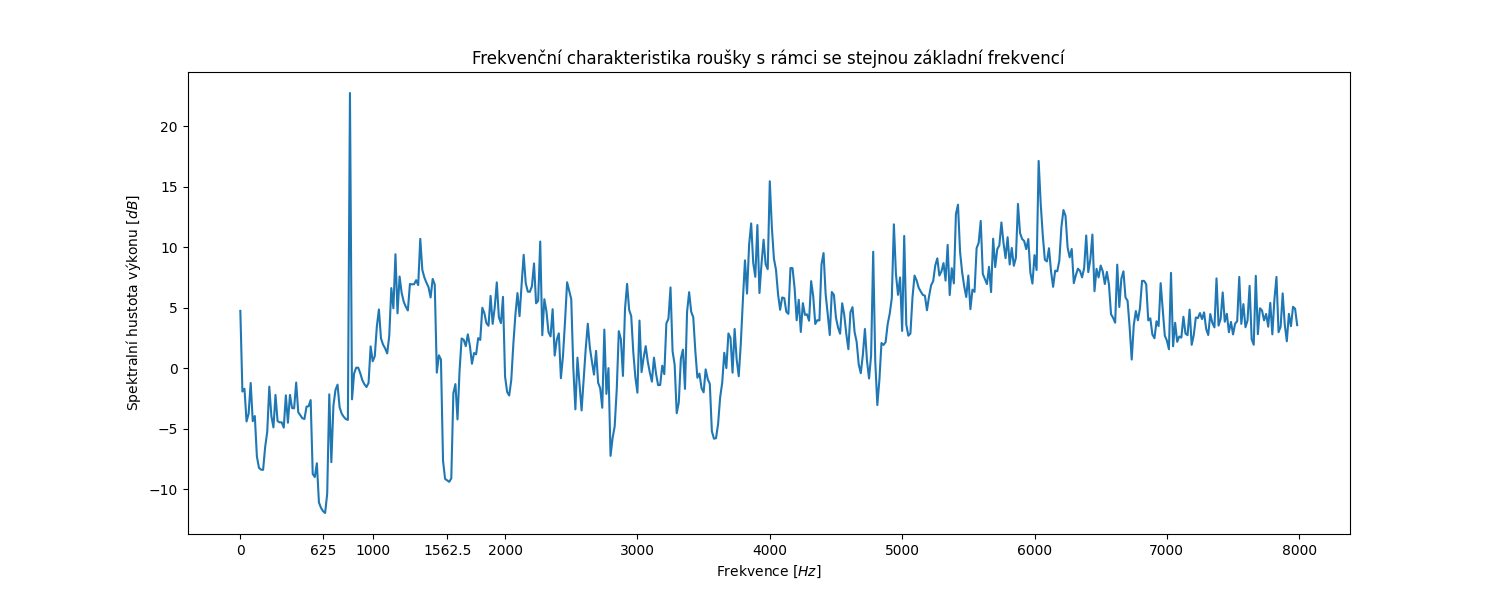
\includegraphics[scale=0.55]{ukol13.png}

\hspace{-4.5em}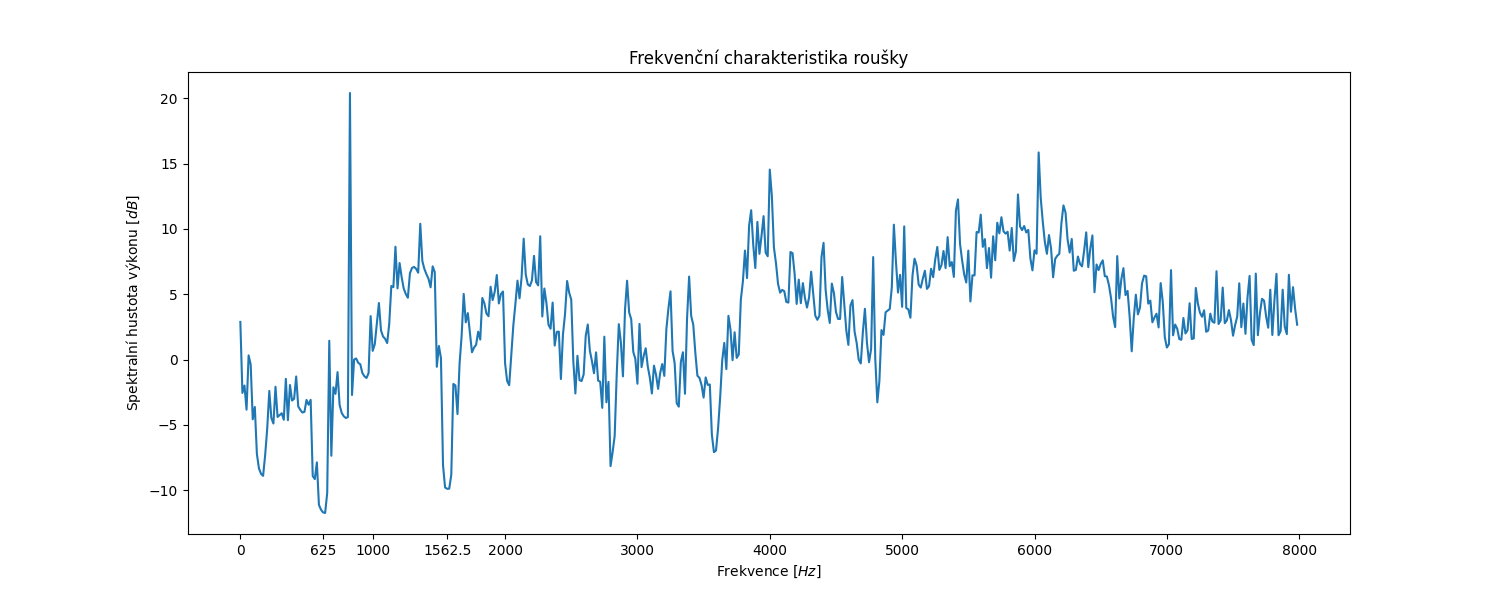
\includegraphics[scale=0.55]{ukol6.png}
\subsection{Neimplementováno}
\newpage
\subsection{Fázový posun}
\hspace{1.5em}Fázový posun jsem řešil způsobem popsaným v zadání. Navíc se mi občas stávalo, že při korelaci docházelo k detekci dvojnásobného posunu (tedy ke stejnému problému jako dvojnásobný lag). Pokud tento problém nastal (oba posuny byly o více než $80$ rámců, tj. více než možný posun), použil jsem pro jeho řešení již známou základní frekvenci. Z frekvence jsem vypočítal délku periody ($T=F_s/f_0$), kterou jsem od obou posunů v absolutní hodnotě odečetl a získal jsem tak správný posun. Posun rámců je implementován funkcí \texttt{phase\_shift()}.

\vspace{1em}
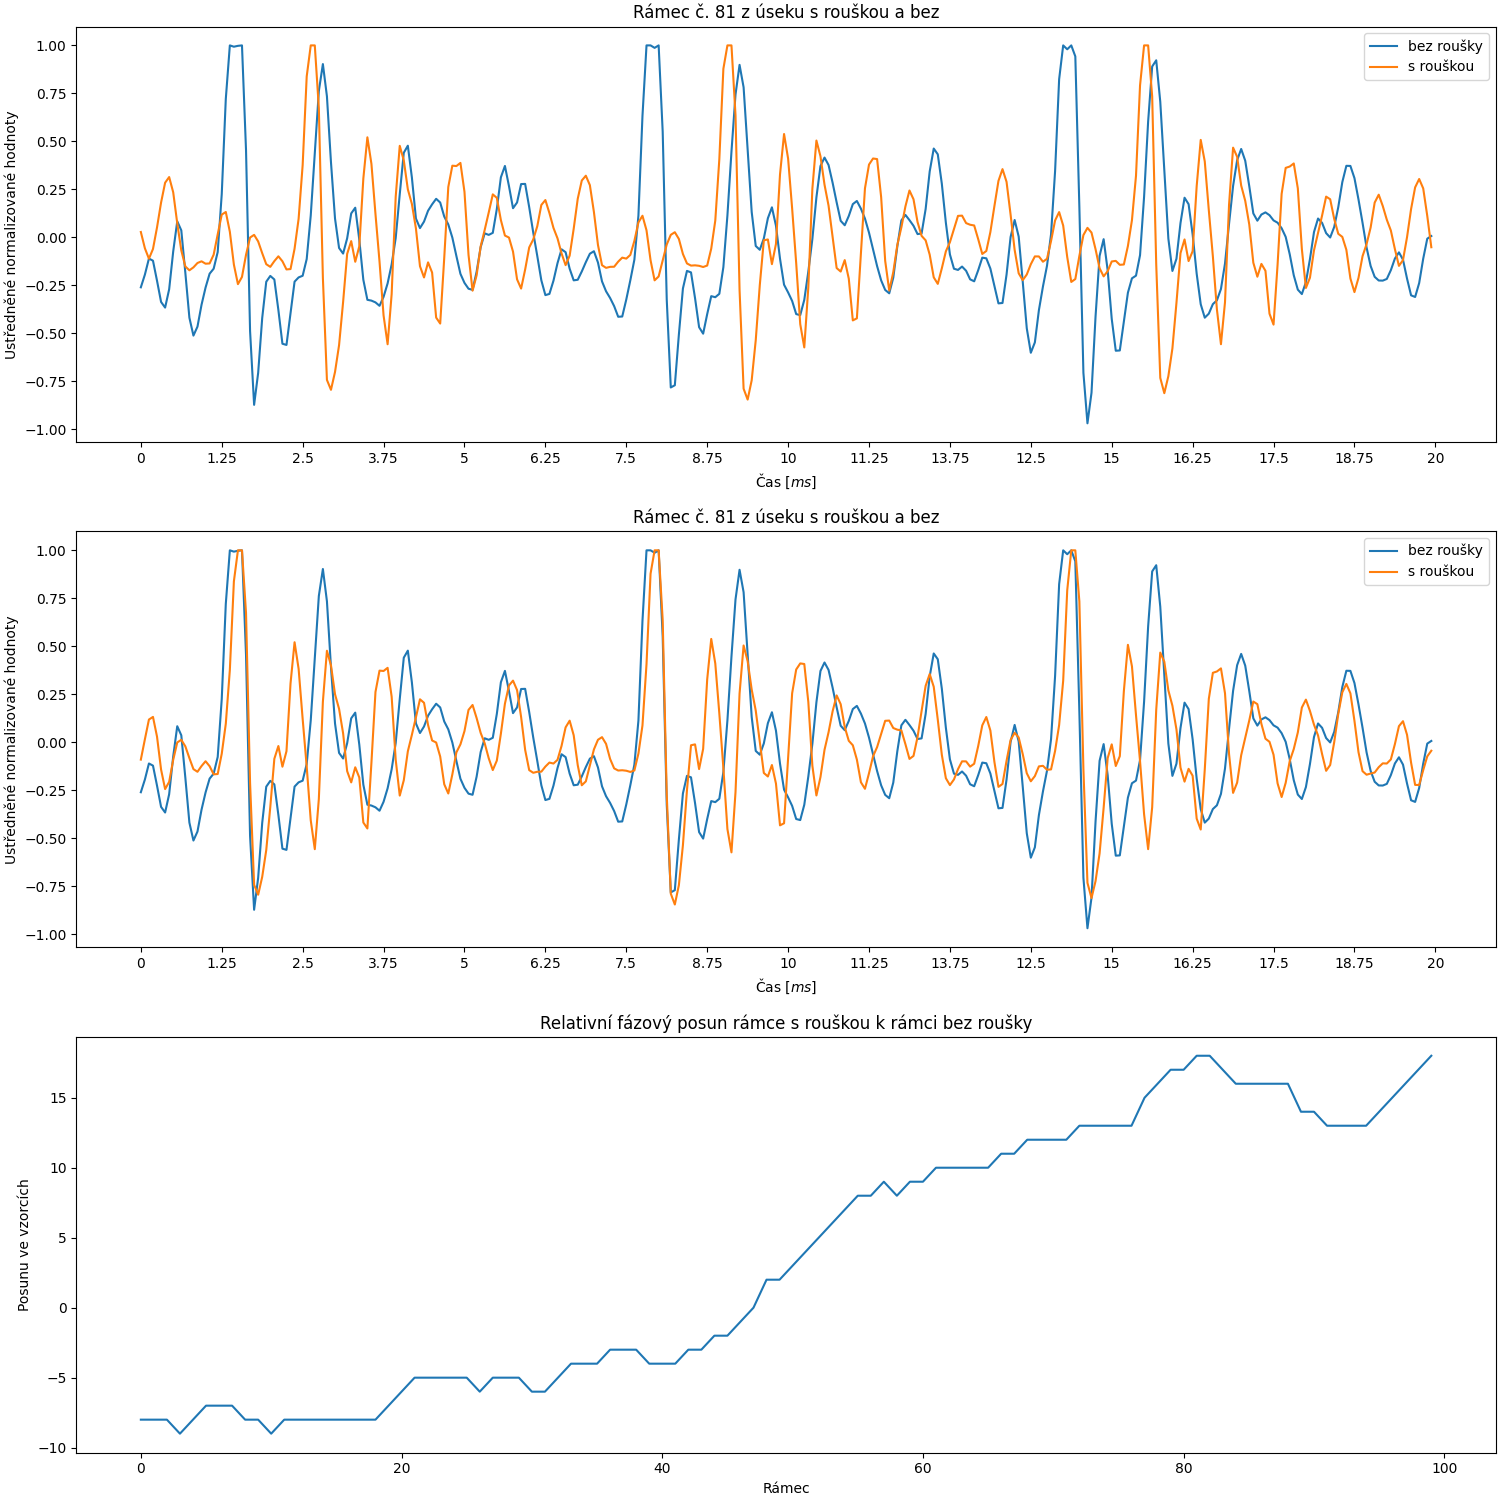
\includegraphics[scale=0.43]{ukol15.png}

\textbf{Bonus:}

\hspace{1.5em}Sečtení fázového posunu na obě strany by nám mělo dát délku periody ve vzorcích. Délka periody by pak měla odpovídat indexu lagu, protože při autokorelaci je si signál sám se sebou nejvíce podobný,´ právě když je posunut o jednu periodu.
\end{document}